%===========================================================================%
%                                                                           %
% This file is part of the documentation for the SYMPHONY MILP Solver.      %
%                                                                           %
% SYMPHONY was jointly developed by Ted Ralphs (ted@lehigh.edu) and         %
% Laci Ladanyi (ladanyi@us.ibm.com).                                        %
%                                                                           %
% (c) Copyright 2000-2015 Ted Ralphs. All Rights Reserved.                  %
%                                                                           %
% SYMPHONY is licensed under the Eclipse Public License. Please see         %
% accompanying file for terms.                                              %
%                                                                           %
%===========================================================================%

\section{Branch and Bound}

{\em Branch and bound} is the broad class of algorithms from which
branch, cut, and price is descended. A branch and bound algorithm uses
a divide and conquer strategy to partition the solution space into
{\em subproblems} and then optimizes individually over each
subproblem. For instance, let $S$ be the set of solutions to a given
problem, and let $c \in {\bf R}^S$ be a vector of costs associated
with members of S. Suppose we wish to determine a least cost member of
S and we are given $\hat{s} \in S$, a ``good'' solution determined
heuristically. Using branch and bound, we initially examine the entire
solution space $S$. In the {\em processing} or {\em bounding} phase,
we relax the problem. In so doing, we admit solutions that are not in
the feasible set $S$. Solving this relaxation yields a lower bound on
the value of an optimal solution. If the solution to this relaxation
is a member of $S$ or has cost equal to $\hat{s}$, then we are
done---either the new solution or $\hat{s}$, respectively, is optimal.
Otherwise, we identify $n$ subsets of $S$, $S_1, \ldots, S_n$, such
that $\cup_{i = 1}^n S_i = S$. Each of these subsets is called a {\em
subproblem}; $S_1, \ldots, S_n$ are sometimes called the {\em
children} of $S$. We add the children of $S$ to the list of {\em
candidate subproblems} (those which need processing). This is called
{\em branching}.

To continue the algorithm, we select one of the candidate subproblems
and process it. There are four possible results. If we find a feasible
solution better than $\hat{s}$, then we replace $\hat{s}$ with the new
solution and continue. We may also find that the subproblem has no
solutions, in which case we discard, or {\em prune} it. Otherwise, we
compare the lower bound to our global upper bound. If it is greater
than or equal to our current upper bound, then we may again prune the
subproblem. Finally, if we cannot prune the subproblem, we are forced
to branch and add the children of this subproblem to the list of
active candidates. We continue in this way until the list of active
subproblems is empty, at which point our current best solution is the
optimal one.

\section{Branch and Cut}
\label{branchandcut}

In many applications, the bounding operation is accomplished using the
tools of linear programming (LP), a technique first described in full
generality by Hoffman and Padberg \cite{hoff:LP}. This general class of
algorithms is known as {\em LP-based branch and bound}. Typically, the
integrality constraints of an integer programming formulation of the
problem are relaxed to obtain a {\em LP relaxation}, which is then
solved to obtain a lower bound for the problem. In \cite{padb:branc},
Padberg and Rinaldi improved on this basic idea by describing a method
of using globally valid inequalities (i.e., inequalities valid for the
convex hull of integer solutions) to strengthen the LP relaxation.
They called this technique {\em branch and cut}. Since then, many
implementations (including ours) have been fashioned around the
framework they described for solving the Traveling Salesman Problem.

\begin{figure}
\framebox[6.5in]{
\begin{minipage}{6.0in}
\vskip .1in
{\rm
{\bf Bounding Operation}\\
\underbar{Input:} A subproblem ${\cal S}$, described in
terms of a ``small'' set of inequalities ${\cal L'}$ such that ${\cal
S} = \{x^s : s \in {\cal F}\;\hbox{\rm and}\;ax^s \leq \beta\;\forall
\;(a,\beta) \in {\cal L'}\}$ and $\alpha$, an upper bound on the global 
optimal value. \\
\underbar{Output:} Either (1) an optimal solution $s^* \in {\cal S}$ to
the subproblem, (2) a lower bound on the optimal value of the 
subproblem, or (3) a message {\tt pruned} indicating that the
subproblem should not be considered further. \\
{\bf Step 1.} Set ${\cal C} \leftarrow {\cal L'}$. \\ 
{\bf Step 2.} Solve the LP $\min\{cx : ax \leq \beta\;\forall\;(a, \beta) 
\in {\cal C}\}$. \\
{\bf Step 3.} If the LP has a feasible solution $\hat{x}$, then go to
Step 4. Otherwise, STOP and output {\tt pruned}. This subproblem has no 
feasible solutions. \\ 
{\bf Step 4.} If $c\hat{x} < \alpha$, then go to Step
5. Otherwise, STOP and output {\tt pruned}. This subproblem
cannot produce a solution of value better than $\alpha$. \\ 
{\bf Step 5.} If $\hat{x}$ is the incidence vector of some $\hat{s}
\in {\cal S}$, then $\hat{s}$ is the optimal solution to this
subproblem. STOP and output $\hat{s}$ as $s^*$. Otherwise, apply
separation algorithms and heuristics to $\hat{x}$ to get a set of
violated inequalities ${\cal C'}$. If ${\cal C'} = \emptyset$, then
$c\hat{x}$ is a lower bound on the value of an optimal element of
${\cal S}$.  STOP and return $\hat{x}$ and the lower bound
$c\hat{x}$. Otherwise, set ${\cal C} \leftarrow {\cal C} \cup {\cal
C'}$ and go to Step 2.}
\end{minipage}
}
\caption{Bounding in the branch and cut algorithm}
\label{proc-bound}
\end{figure}
As an example, let a combinatorial optimization problem $\hbox{\em CP} =
(E, {\cal F})$ with {\em ground set} $E$ and {\em feasible set} ${\cal F}
\subseteq 2^E$ be given along with a cost function $c \in {\bf R}^E$.
The incidence vectors corresponding to the members of ${\cal F}$ are
sometimes specified as the the set of all incidence vectors obeying a
(relatively) small set of inequalities. These inequalities are
typically the ones used in the initial LP relaxation. Now let ${\cal
P}$ be the convex hull of incidence vectors of members of ${\cal
F}$. Then we know by Weyl's Theorem (see \cite{nemwol88}) that there exists
a finite set ${\cal L}$ of inequalities valid for ${\cal P}$ such that
\begin{equation}
\label{the-polyhedron}
{\cal P} = \{x \in {\bf R}^n: ax \leq \beta\;\;\forall\;(a, \beta) \in 
{\cal L}\}.
\end{equation}
The inequalities in ${\cal L}$ are the potential cutting planes to be
added to the relaxation as needed. Unfortunately, it is usually
difficult, if not impossible, to enumerate all of inequalities in
${\cal L}$ or we could simply solve the problem using linear
programming. Instead, they are defined implicitly and we use
separation algorithms and heuristics to generate these inequalities
when they are violated. In Figure \ref{proc-bound}, we describe more
precisely how the bounding operation is carried out in branch and cut.
\begin{figure}
\framebox[6.5in]{
\begin{minipage}{6.0in}
\vskip .1in
{\rm
{\bf Branching Operation} \\
\underbar{Input:} A subproblem ${\cal S}$ and $\hat{x}$, the LP solution
yielding the lower bound. \\
\underbar{Output:} $S_1, \ldots, S_p$ such that ${\cal S} = \cup_{i = 1}^p
S_i$. \\
{\bf Step 1.} Determine sets ${\cal L}_1, \ldots, {\cal L}_p$ of
inequalities such that ${\cal S} = \cup_{i = 1}^n \{x \in {\cal S}: ax \leq
\beta\;\forall\;(a, \beta) \in {\cal L}_i\}$ and $\hat{x} \notin
\cup_{i = 1}^n S_i$. \\
{\bf Step 2.} Set $S_i = \{x \in {\cal S}: ax \leq
\beta\;\;\forall\;(a, \beta) \in {\cal L}_i \cup {\cal L}'\}$ where 
${\cal L'}$ is the set of inequalities used to describe ${\cal S}$.}
\end{minipage}
}
\caption{Branching in the branch and cut algorithm}
\label{branching-fig}
\end{figure}

\indent Once we have failed to either prune the current subproblem or separate
the current fractional solution from ${\cal P}$, we are forced to
branch. The branching operation is accomplished by specifying a set of
hyperplanes which divide the current subproblem in such a way that the
current solution is not feasible for the LP relaxation of any of the
new subproblems. For example, in a combinatorial optimization problem,
branching could be accomplished simply by fixing a variable whose
current value is fractional to 0 in one branch and 1
in the other. The procedure is described more formally in Figure
\ref{branching-fig}. Figure \ref{gb&c} gives a high level description
of the generic branch and cut algorithm.
\begin{figure}
\framebox[6.5in]{
\begin{minipage}{6.0in}
\vskip .1in
{\rm
{\bf Generic Branch and Cut Algorithm}\\
\underbar{Input:} A data array specifying the problem instance.\\
\underbar{Output:} The global optimal solution $s^*$ to the problem
instance. \\
{\bf Step 1.} Generate a ``good'' feasible solution ${\hat s}$ using 
heuristics. Set $\alpha \leftarrow c(\hat{s})$. \\
{\bf Step 2.} Generate the first subproblem ${\cal S}^I$ by constructing a
small set ${\cal L'}$ of inequalities valid for ${\cal P}$. Set $A
\leftarrow \{{\cal S}^I\}$. \\
{\bf Step 3.} If $A = \emptyset$, STOP and output $\hat{s}$ as the
global optimum $s^*$. Otherwise, choose some ${\cal S} \in A$. Set $A
\leftarrow A \setminus \{{\cal S}\}$. Process ${\cal S}$. \\
{\bf Step 4.} If the result of Step 3 is a feasible solution
$\overline{s}$, then $c\overline{s} < c\hat{s}$.
Set $\hat{s} \leftarrow \overline{s}$ and $\alpha \leftarrow 
c(\overline{s})$ and go to Step 3. If the subproblem was pruned, go to
Step 3. Otherwise, go to Step 5. \\
{\bf Step 5.} Perform the branching operation. Add the set of
subproblems generated to $A$ and go to Step 3.}
\end{minipage}
}
\caption{Description of the generic branch and cut algorithm}
\label{gb&c}
\end{figure}

In the remainder of the manual, we often use the term {\em search
tree}. This term derives from the common representation of the list of
subproblems as the nodes of a graph in which each subproblem is
connected only to its parent and its children. Storing the subproblems
in such a form is an important aspect of our global data structures.
Since the subproblems correspond to the nodes of this graph, they are
sometimes be referred to as {\em nodes in the search tree} or simply
as {\em nodes}. The {\em root node} or {\em root} of the tree is the
node representing the initial subproblem.

\section{Design of SYMPHONY}
\label{design}

\BB\ was designed with two major goals in mind---portability and
ease of use. With respect to ease of use, we aimed for a ``black box''
design, whereby the user would not be required to know anything about
the implementation of the library, but only about the user interface.
With respect to portability, we aimed not only for it to be {\em
possible} to use the framework in a wide variety of settings and on a
wide variety of hardware, but also for it to perform {\em effectively} in all
these settings. Our primary measure of effectiveness was
how well the framework would perform in comparison to a problem-specific
(or hardware-specific) implementation written ``from scratch.''

It is important to point out that achieving such design goals involves
a number of very difficult tradeoffs. For instance, ease of use is quite
often at odds with efficiency. In several instances, we had to give up
some efficiency to make the code easy to work with and to maintain a
true black box implementation. Maintaining portability across a wide
variety of hardware, both sequential and parallel, also required some
difficult choices. For example, solving large-scale problems on
sequential platforms requires extremely memory-efficient data
structures in order to maintain the very large search trees that can
be generated. These storage schemes, however, are highly centralized
and do not scale well to large numbers of processors. 

\subsection{An Object-oriented Approach}

As we have already alluded to, applying BCP to large-scale problems
presents several difficult challenges. First and foremost is designing
methods and data structures capable of handling the potentially huge
numbers of cuts and variables that need to be accounted for during the
solution process. The dynamic nature of the algorithm requires that we
must also be able to efficiently move cuts and variables in and out of
the {\em active set} of each search node at any time. A second,
closely-related challenge is that of effectively dealing with the very
large search trees that can be generated for difficult problem
instances. This involves not only the important question of how to
store the data, but also how to move it between modules during
parallel execution. A final challenge in developing a generic
framework, such as SYMPHONY, is to deal with these issues using a
problem-independent approach.

Describing a node in the search tree consists of, among other things,
specifying which cuts and variables are initially {\em active} in the
subproblem. In fact, the vast majority of the methods in BCP that
depend on the model are related to generating, manipulating, and
storing the cuts and variables. Hence, SYMPHONY can be considered an
object-oriented framework with the central ``objects'' being the cuts
and variables. From the user's perspective, implementing a BCP
algorithm using SYMPHONY consists primarily of specifying various
properties of objects, such as how they are generated, how they are
represented, and how they should be realized within the context of a
particular subproblem.

With this approach, we achieved the ``black box'' structure by
separating these problem-specific functions from the rest of the
implementation. The internal library interfaces with the user's
subroutines through a well-defined Application Program Interface (API) (see
Section \ref{API})
and independently performs all the normal functions of BCP---tree
management, LP solution, and cut pool management, as well as inter-process
communication (when parallelism is employed). Although there are
default options for many of the operations, the user can also assert
control over the behavior of the algorithm by overriding the default
methods or by parameter setting.

Although we have described our approach as being ``object-oriented,''
we would like to point out that SYMPHONY is implemented in C, not C++.
To avoid inefficiencies and enhance the modularity of the code
(allowing for easy parallelization), we used a more
``function-oriented'' approach for the implementation of certain
aspects of the framework. For instance, methods used for communicating
data between modules are not naturally ``object-oriented'' because the
type of data being communicated is usually not known by the
message-passing interface. It is also common that efficiency
considerations require that a particular method be performed on a
whole set of objects at once rather than on just a single object.
Simply invoking the same method sequentially on each of the members of
the set can be extremely inefficient. In these cases, it is far better
to define a method which operates on the whole set at once. In order
to overcome these problems, we have also defined a set of {\em
interface functions}, which are associated with the computational
modules. These function is described in detail in Section \ref{API}.

\subsection{Data Structures and Storage}
\label{data-structures}

Both the memory required to store the search tree and the time
required to process a node are largely dependent on the number of
objects (cuts and variables) that are active in each subproblem.
Keeping this active set as small as possible is one of the keys to
efficiently implementing BCP. For this reason, we chose data
structures that enhance our ability to efficiently move objects in and
out of the active set. Allowing sets of cuts and variables to move in
and out of the linear programs simultaneously is one of the most
significant challenges of BCP. We do this by maintaining an abstract
{\em representation} of each global object that contains information
about how to add it to a particular LP relaxation. 

In the literature on linear and integer programming, the terms {\em
cut} and {\em row} are typically used interchangeably. Similarly, {\em
variable} and {\em column} are often used with similar meanings. In
many situations, this is appropriate and does not cause confusion.
However, in object-oriented BCP frameworks, such as \BB\ or ABACUS
\cite{abacus1}, a {\em cut} and a {\em row} are {\em fundamentally
different objects}. A {\em cut} (also referred to as a {\em
constraint}) is a user-defined representation of an abstract object
which can only be realized as a row in an LP matrix {\em with respect
to a particular set of active variables}. Similarly, a {\em variable}
is a representation which can only be realized as a column of an LP
matrix with respect to a {\em particular set of cuts}. This
distinction between the {\em representation} and the {\em realization}
of objects is a crucial design element and is what allows us to
effectively address some of the challenges inherent in BCP. In the
remainder of this section, we further discuss this distinction
and its implications.

%In later sections, we will discuss the computational issues involved
%in the efficient processing of individual subproblem.

\subsubsection{Variables}
\label{variables}

In \BB, problem variables are {\em represented} by a unique global
index assigned to each variable by the user. This index represents
each variable's position in a ``virtual'' global list known only to
the user. The main requirement of this indexing scheme is that, given
an index and a list of active cuts, the user must be able to generate
the corresponding column to be added to the matrix. As an example, in
problems where the variables correspond to the edges of an underlying
graph, the index could be derived from a lexicographic ordering of the
edges (when viewed as ordered pairs of nodes).

This indexing scheme provides a very compact representation, as well
as a simple and effective means of moving variables in and out of the
active set. However, it means that the user must have a priori
knowledge of all problem variables and a method for indexing them. For
combinatorial models such as the {\em Traveling Salesman Problem},
this does not present a problem. However, for some set partitioning
models, for instance, the number of columns may not be known in
advance. Even if the number of columns is known in advance, a viable
indexing scheme may not be evident. Eliminating the indexing
requirement by allowing variables to have abstract, user-defined
representations (such as we do for cuts), would allow for more
generality, but would also sacrifice some efficiency. A hybrid scheme,
allowing the user to have both indexed and {\em algorithmic} variables
(variables with user-defined representations) is planned for a future 
version of SYMPHONY.

For efficiency, the problem variables can be divided into two sets, the
{\em base variables} and the {\em extra variables}. The base variables
are active in all subproblems, whereas the extra variables can be
added and removed. There is no theoretical difference between
base variables and extra variables; however, designating a well-chosen
set of base variables can significantly increase efficiency. Because
they can move in and out of the problem, maintaining extra variables
requires additional bookkeeping and computation. If the user has
reason to believe a priori that a variable is ``good'' or has a high
probability of having a non-zero value in some optimal solution to the
problem, then that variable should be designated as a base variable.
It is up to the user to designate which variables should be active in
the root subproblem. Typically, when column generation is used, only base 
variables are active. Otherwise, all variables must be active in the 
root node.

\subsubsection{Constraints}
\label{constraints}

Because the global list of potential constraints (also called cuts) is
not usually known a priori or is extremely large, constraints cannot
generally be represented simply by a user-assigned index. Instead,
each constraint is assigned a global index only after it becomes
active in some subproblem. It is up to the user, if desired, to
designate a compact {\em representation} for each class of constraints
that is to be generated and to implement subroutines for converting
from this compact representation to a matrix row, given the list of
active variables. For instance, suppose that the set of nonzero
variables in a particular class of constraints corresponds to the set
of edges across a cut in a graph. Instead of storing the indices of
each variable explicitly, one could simply store the set of nodes on
one side (``shore'') of the cut as a bit array. The constraint could
then be constructed easily for any particular set of active variables
(edges).

Just as with variables, the constraints are divided into {\em core
constraints} and {\em extra constraints}. The core constraints are
those that are active in every subproblem, whereas the extra
constraints can be generated dynamically and are free to enter and leave
as appropriate. Obviously, the set of core constraints must be known
and constructed explicitly by the user. Extra constraints, on the
other hand, are generated dynamically by the cut generator as they are
violated. As with variables, a good set of core constraints can have a
significant effect on efficiency.

Note that the user is not {\em required} to designate a compact
representation scheme. Constraints can simply be represented
explicitly as matrix rows with respect to the global set of variables.
However, designating a compact form can result in large reductions in
memory use if the number of variables in the problem is large.

\subsubsection{Search Tree}

Having described the basics of how objects are represented, we now
describe the representation of search tree nodes. Since the base
constraints and variables are present in every subproblem, only the
indices of the extra constraints and variables are stored in each
node's description. A complete description of the current basis is
maintained to allow a warm start to the computation in each search
node. This basis is either inherited from the parent, computed during
strong branching (see Section \ref{branching}), or comes from earlier
partial processing of the node itself (see Section \ref{two-phase}).
Along with the set of active objects, we must also store the identity
of the object(s) which were branched upon to generate the node. The
branching operation is described in Section \ref{branching}.

Because the set of active objects and the status of the basis do not
tend to change much from parent to child, all of these data are stored
as differences with respect to the parent when that description is
smaller than the explicit one. This method of storing the entire tree
is highly memory-efficient. The list of nodes that are candidates for
processing is stored in a heap ordered by a comparison function
defined by the search strategy (see \ref{tree-management}). This
allows efficient generation of the next node to be processed.

\subsection{Modular Implementation}
\label{SYMPHONY-modules}

\BB's functions are grouped into five independent computational
modules. This modular implementation not only facilitates code
maintenance, but also allows easy and highly configurable
parallelization. Depending on the computational setting, the modules
can be compiled as either (1) a single sequential code, (2) a
multi-threaded shared-memory parallel code, or (3) separate processes
running in distributed fashion over a network. The modules pass data
to each other either through shared memory (in the case of sequential
computation or shared-memory parallelism) or through a message-passing
protocol defined in a separate communications API (in the case of
distributed execution). an schematic overview of the modules is
presented in Figure \ref{overview}. In the remainder of the section,
we describe the modularization scheme and the implementation of each
module in a sequential environment. 

\begin{figure}
\centering
%\psfig{figure=pbandc.eps}
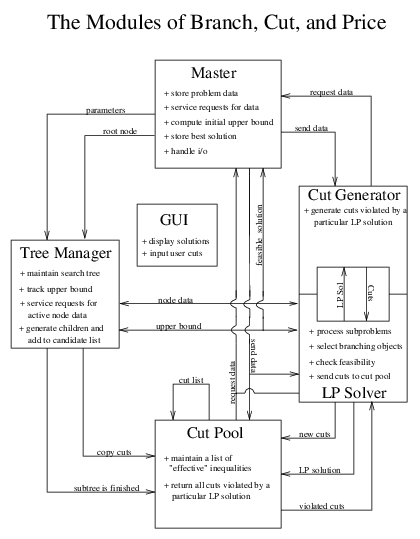
\includegraphics{pbandc}
\caption{Schematic overview of the branch, cut, and price algorithm}
\label{overview}
\end{figure}

\subsubsection{The Master Module}
\label{master-process}

The {\em master module} includes functions that perform problem initialization
and I/O. This module is the only persistent module and stores all static
problem data. The other modules are created only during a solve call and
destroyed afterward. All calls to the API are processed through the master
module. These functions of the master module implement the following tasks:
%\underbar{Overall Function:} Handle input/output, maintain the data
%for the problem instance and serve requests to send out that
%data. Keep track of the best solution found so far.\\
%\underbar{Specific Functions:}
\begin{itemize}
        \item Initialize the environment.
        \item Set and maintain parameter values.
        \item Read and store static problem data for instance to be solved.
        \item Compute an initial upper bound using heuristics.
        \item Perform problem preprocessing.
        \item Initialize the solution process, pass problem information to the
        solver modules and store the results after completion of the solve 
	call.
        \item Track the status of associated processes during parallel
        solution calls.
        \item Act as a clearing house for output during the solution process.
        \item Store warm start information between solver calls.
        \item Service requests from the user through the API for problem data,
        problem modification, and parameter modification.
\end{itemize}

\subsubsection{The Tree Management Module}

The \emph{tree manager} controls the overall execution of the algorithm. It
tracks the status of its worker modules, as well as that of the search
tree, and distributes the subproblems to be processed to the node processing
module(s). Functions performed by the tree management module are:
%\underbar{Overall Function:} Start up all the processes and keep
%track of the current state of the search tree.
%\noindent \underbar{Specific Functions:} \nobreak
\begin{itemize}
        \item Receive data for the root node and place it on the list 
        of candidates for processing.
        \item Receive data for subproblems to be held for later
        processing.
        \item Handle requests from linear programming modules to
        release a subproblem for processing.
        \item Receive branching object information, set up data structures
        for the children, and add them to the list of candidate subproblems.
        \item Keep track of the global upper bound and notify all node
        processing modules when it changes.
        \item Write current state information out to disk periodically
        to allow a restart in the event of a system crash.
        \item Keep track of run data and send it to the master
        program at termination.
\end{itemize} 

\subsubsection{The Node Processing Module}

The \emph{node processing} (NP) module is the most complex and
computationally intensive of the five processes. Its job is to perform
the bounding and branching operations. These operations
are, of course, central to the performance of the algorithm. Functions
performed by the LP module are:
%\underbar{Overall Function:} Process and bound subproblems. Branch and
%produce new subproblems. \\
%\underbar{Specific Functions:} 
\begin{itemize}
        \item Inform the tree manager when a new subproblem is needed.
        \item Receive a subproblem and process it in conjunction
        with the cut generator and the cut pool.
        \item Decide which cuts should be sent to the global pool to
        be made available to other NP modules.
        \item If necessary, choose a branching object and send its
        description back to the tree manager.
        \item Perform the fathoming operation, including generating
        variables. 
\end{itemize} 

\subsubsection{The Cut Generation Module}

The {\em cut generator} performs only one function---generating valid
inequalities violated by the current fractional solution and sending
them back to the requesting LP process. Here are the functions
performed by the cut generator module:
%\underbar{Overall Function:} Receive solution vectors from the LP
%processes and generate valid inequalities violated by these vectors.\\
%\underbar{Specific Functions:}
\begin{itemize}
        \item Receive an LP solution and attempt to
        separate it from the convex hull of all solutions.
        \item Send generated valid inequalities back to the NP module.  
        \item When finished processing a solution vector, inform the
        NP module not to expect any more cuts in case it is still waiting.
\end{itemize}

\subsubsection{The Cut Management Module}

The concept of a {\em cut pool} was first suggested by Padberg and
Rinaldi \cite{padb:branc}, and is based on the observation that in BCP, the
inequalities which are generated while processing a particular node in
the search tree are also generally valid and potentially useful at
other nodes. Since generating these cuts is usually a relatively
expensive operation, the cut pool maintains a list of the ``best'' or
``strongest'' cuts found in the tree so far for use in processing
future subproblems. Hence, the cut manager functions as an auxiliary cut
generator. More explicitly, here are the functions of the cut pool
module:
%\underbar{Overall Function:} Maintain a list of ``effective'' valid
%inequalities for use in processing the subproblems.\\
%\underbar{Specific Functions:}
\begin{itemize}
        \item Receive cuts generated by other modules and store them.
        \item Receive an LP solution and return a
set of cuts which this solution violates.
        \item Periodically purge ``ineffective'' and duplicate cuts
to control its size.
\end{itemize}

\subsection{Algorithm Summary}
\label{symphony}

Currently, \BB\ is what is known as a single-pool BCP algorithm.
The term {\em single-pool} refers to the fact that there is a single
central list of candidate subproblems to be processed, which is
maintained by the tree manager. Most sequential implementations use
such a single-pool scheme. However, other schemes may be used in
parallel implementations. For a description of various types of
parallel branch and bound, see \cite{gend:paral}.

The user begins by initializing the SYMPHONY environment and can then invoke
subroutines for reading in parameters and problem data, finding an initial
upper bound, and designating the initial set of active cuts and variables in
the root node. Once the user invokes a solve routine, a tree manager is
created to manage the solution process. The tree manager module in turn sets
up the cut pool module(s), the linear programming module(s), and the cut
generator module(s). Currently, there are three solve calls supported by the
API. The first call is the \emph{initial solve} (see Section
\ref{initial_solve}), which solves the problem from scratch without using warm
start information. The second type of solve call is a \emph{warm solve}, which
solves the problem using previously computed warm start information (see
Section \ref{warm_solve}). Finally, there is a \emph{multicriteria solve} call
which is used to enumerate efficient solutions to a given multicriteria MILP
(see Section \ref{mc_solve}).

During the solution process, the tree manager functions control the execution
by maintaining the list of candidate subproblems and sending them to the NP
modules as they become idle. The NP modules receive nodes from the tree
manager, process them, branch (if required), and send back the identity of the
chosen branching object to the tree manager, which in turn generates the
children and places them on the list of candidates to be processed (see
Section \ref{branching} for a description of the branching operation). A
schematic summary of the algorithm is shown in Figure \ref{overview}. The
preference ordering for processing nodes is a run-time parameter. Typically,
the node with the smallest lower bound is chosen to be processed next since
this strategy minimizes the overall size of the search tree. However, at
times, it is advantageous to {\em dive} down in the tree. The concepts of {\em
diving} and {\em search chains}, introduced in Section \ref{tree-management},
extend the basic ``best-first'' approach.

We mentioned earlier that cuts and variables can be treated in a
somewhat symmetric fashion. However, it should be clear by now
that our current implementation favors the implementation of
branch and cut algorithms, where the computational effort spent
generating cuts dominates that of generating variables. Our methods of
representation also clearly favor such problems. In a future version
of the software, we plan to erase this bias by adding additional
functionality for handling variable generation and storage. This is
the approach already taken by of COIN/BCP \cite{coin-or}. For more
discussion of the reasons for this bias and the differences between
the treatment of cuts and variables, see Section \ref{lp-relaxation}.

\section{Details of the Implementation}
\label{modules}

\subsection{The Master Module}
\label{master}

The primary functions performed by the master module were listed in
Section \ref{master-process}. Here, we describe the implementational details of
the various solve calls.  
%If needed, the user must provide a
%routine to read problem-specific parameters in from the parameter
%file. She must also provide a subroutine for upper bounding if
%desired, though upper bounds can also be provided explicitly. A good
%initial upper bound can dramatically decrease the solution time by
%allowing more variable-fixing and earlier pruning of search tree
%nodes. If no upper bounding subroutine is available, then the
%two-phase algorithm, in which a good upper bound is found quickly in
%the first phase using a reduced set of variables can be advantageous.
%See Section \ref{two-phase} for details. The user's only unavoidable
%obligation during pre-processing is to specify the list of base
%variables and, if desired, the list of extra variables that are to be
%active in the root node. Again, we point out that selecting a good set
%of base variables can make a marked difference in solution speed,
%especially using the two-phase algorithm.

\subsubsection{Initial Solve}\label{initial_solve}

Calling the initial solve method solves a given MILP from scratch, as
described above. The first action taken is to create an instance of the tree
manager module that will control execution of the algorithm. If the algorithm
is to be executed in parallel on a distributed architecture, the master module
spawns a separate tree manager process that will autonomously control the
solution process. The tree manager in turn creates the modules for processing
the nodes of the search tree, generating cuts, and maintaining cut pools.
These modules work in concert to execute the solution process. When it makes
sense, sets of two or more modules, such as a node processing module and a cut
generation module may be combined to yield a single process in which the
combined modules work in concert and communicate with each other through
shared memory instead of across the network. When running as separate process,
the modules communicate with each other using a standard communications
protocol. Currently, the only option supported is PVM, but it would be
relatively easy to add an MPI implementation.

The overall flow of the algorithm is similar to other branch and bound
implementations and is detailed below. A priority queue of candidate
subproblems available for processing is maintained at all times and the
candidates are processed in an order determined by the search strategy. The
algorithm terminates when the queue is empty or when another specified
condition is satisfied. A new feature in SYMPHONY \VER\  is the ability to stop
the computation based on exceeding a given time limit, exceeding a given limit
on the number of processed nodes, achieving a target percentage gap between
the upper and lower bounds, or finding the first feasible solution. After
halting prematurely, the computation can be restarted after modifying
parameters or problem data. This enables the implementation of a wide range of
dynamic and on-line solution algorithms, as we describe next.

\subsubsection{Solve from Warm Start} \label{warm_solve}

Among the utility classes in the COIN-OR repository is a base class for
describing the data needed to warm start the solution process for a particular
solver or class of solvers. To support this option for SYMPHONY, we have
implemented such a warm start class for MILPs. The main content of the class
is a compact description of the search tree at the time the computation was
halted. This description contains complete information about the subproblem
corresponding to each node in the search tree, including the branching
decisions that lead to the creation of the node, the list of active variables
and constraints, and warm start information for the subproblem itself (which
is a linear program). All information is stored compactly using SYMPHONY's
native data structures, which store only the differences between a child and
its parent, rather than an explicit description of every node. This approach
reduces the tree's description to a fraction of the size it would otherwise
be. In addition to the tree itself, other relevant information regarding the
status of the computation is recorded, such as the current bounds and best
feasible solution found so far. Using the warm start class, the user can save
a warm start to disk, read one from disk, or restart the computation at any
point after modifying parameters or the problem data itself. This allows
the user to easily implement periodic checkpointing, to design dynamic
algorithms in which the parameters are modified after the gap reaches a
certain threshold, or to modify problem data during the solution process if
needed.

\paragraph{Modifying Parameters.}

The most straightforward use of the warm start class is to restart the solver
after modifying problem parameters. To start the computation from a given warm
start when the problem data has not been modified, the tree manager simply
traverses the tree and adds those nodes marked as candidates for processing to
the node queue. Once the queue has been reformed, the algorithm is then able
to pick up exactly where it left off. Code for using the resolve command was
shown in Figure \ref{dynamic}. The situation is more challenging if the user
modifies problem data in between calls to the solver. We address this
situation next.

\paragraph{Modifying Problem Data.}

If the user modifies problem data in between calls to the solver, SYMPHONY
must make corresponding modifications to the leaf nodes of the current search
tree to allow execution of the algorithm to continue. In principle, any change
to the original data that does not invalidate the subproblem warm start data,
i.e., the basis information for the LP relaxation, can be
accommodated. Currently, SYMPHONY can only handle modifications to the rim
vectors of the original MILP. Methods for handling other modifications, such as
the addition of columns or the modification of the constraint matrix itself,
will be added in the future. To initialize the algorithm, each leaf node,
regardless of its status after termination of the previous solve call, must be
inserted into the queue of candidate nodes and reprocessed with the changed
rim vectors. After this reprocessing, the computation can continue as usual.
Optionally, the user can ``trim the tree'' before resolving. This consists of
locating nodes whose descendants are all likely to be pruned in the resolve
and eliminating those descendants in favor of processing the parent node
itself. This ability could be extended to allow changes that invalidate the
warm start data of some leaf nodes.

The ability to resolve after modifying problem data has a wide range of
applications in practice. One obvious use is to allow dynamic modification of
problem data during the solve procedure, or even after the procedure has been
completed. Implementing such a solver is simply a matter of periodically
stopping to check for user input describing a change to the problem. Another
obvious application is in situations where it is known a priori that the user
will be solving a sequence of very similar MILPs. This occurs, for instance,
when implementing algorithms for multicriteria optimization, as we describe in
Section \ref{mc_solve}. One approach to this is to solve a given ``base
problem'' (possibly limiting the size of the warm start tree), save the warm
start information from the base problem and then start each subsequent call
from this same checkpoint. Code for implementing this was shown in Figure
\ref{warm_start}. 

\subsubsection{Bicriteria Solve}\label{mc_solve}

For those readers not familiar with bicriteria integer programming, we briefly
review the basic notions here. For clarity, we restrict the discussion here to
pure integer programs (ILPs), but the principles are easily generalized. A
bicriteria ILP is a generalization of a standard ILP presented earlier that
includes a second objective function, yielding an optimization problem of the
form
\begin{equation}
\begin{array}{lrcl}
\vmin & [cx, dx],  \label{bicrit} \\
\textrm{s.t.} & Ax & \leq & b, \\ 
& x & \in & \Z^{n}.
\end{array}
\end{equation}
The operator \emph{vmin} is understood to mean that solving this program is
the problem of generating \emph{efficient} solutions, which are these feasible
solutions $p$ to \ref{bicrit} for which there does not exist a second
distinct feasible solution $q$ such that $cq \leq cp$ and $dq \leq dp$ and at
least one inequality is strict. Note that (\ref{bicrit}) does not have a
unique optimal solution value, but a set of pairs of solution values called
\emph{outcomes}. The pairs of solution values corresponding to efficient
solutions are called \emph{Pareto outcomes}. Surveys of methodology for for
enumerating the Pareto outcomes of multicriteria integer programs are provided
by Climaco et al.~\cite{climaco97} and more recently by Ehrgott and
Gandibleux~\cite{ehrgott00, ehrgott02} and Ehrgott and
Wiecek~\cite{ehrgott04}.

The bicriteria ILP (\ref{bicrit}) can be converted to a standard ILP by
taking a nonnegative linear combination of the objective
functions~\cite{geoff68}. Without loss of generality, the weights can be
scaled so they sum to one, resulting in a family of ILPs parameterized by a
scalar $0 \leq \alpha \leq 1$, with the bicriteria objective function replaced
by the \emph{weighted sum objective}
\begin{equation}\label{wsum}
(\alpha c + (1 - \alpha) d) x.
\end{equation}
Each selection of weight $\alpha$ produces a different single-objective
problem. Solving the resulting ILP produces a Pareto outcome called a
\emph{supported outcome}, since it is an extreme point on the convex lower
envelope of the set of Pareto outcomes. Unfortunately, not all efficient
outcomes are supported, so it is not possible to enumerate the set of Pareto
outcomes by solving a sequence of ILPs from this parameterized family. To
obtain all Pareto outcomes, one must replace the weighted sum objective
(\ref{wsum}) with an objective based on the \emph{weighted Chebyshev norm}
studied by Eswaran et al.~\cite{eswaran89} and Solanki~\cite{solanki91}. If
$x^c$ is a solution to a weighted sum problem with $\alpha = 1$ and $x^d$ is
the solution with $\alpha = 0$, then the weighted Chebyshev norm of a feasible
solution $p$ is
\begin{equation}
\max \{\alpha (cp - cx^c), (1 - \alpha)(dp - dx^d)\}.
\label{chebyshev}
\end{equation} 
Although this objective function is not linear, it can easily be linearized by
adding an artificial variable, resulting in a second parameterized family of
ILPs. Under the assumption of \emph{uniform dominance}, Bowman showed that an
outcome is Pareto if and only if it can be obtained by solving some ILP in
this family~\cite{bowman76}. In \cite{WCN}, the authors presented a method for
enumerating all Pareto outcomes by solving a sequence of ILPs in this
parameterized family. By slightly perturbing the objective function, they also
showed how to relax the uniform dominance assumption. Note that the set of all
supported outcomes, which can be thought of as an approximation of the set of
Pareto outcomes, can be similarly obtained by solving a sequence of ILPs with
weighted sum objectives.

SYMPHONY \VER\  contains a generic implementation of the algorithm described in
\cite{WCN}, along with a number of methods for approximating the set of Pareto
outcomes. To support these capabilities, we have extended the OSI interface so
that it allows the user to define a second objective function. Of course, we
have also added a method for invoking this bicriteria solver called
\texttt{multiCriteriaBranchAndBound()}. Relaxing the uniform dominance
requirement requires the underlying ILP solver to have the ability to
generate, among all optimal solutions to a ILP with a primary objective, a
solution minimizing a given secondary objective. We added this capability to
SYMPHONY through the use of optimality cuts, as described in \cite{WCN}.

Because implementing the algorithm requires the solution of a sequence of
ILPs that vary only in their objective functions, it is possible to use warm
starting to our advantage.  Although the linearization of (\ref{chebyshev})
requires modifying the constraint matrix from iteration to iteration, it is
easy to show that these modifications cannot invalidate the basis. In the case
of enumerating all supported outcomes, only the objective function is modified
from one iteration to the next. In both cases, we save warm start information
from the solution of the first ILP in the sequence and use it for each
subsequent computation.

\subsection{The Node Processing Module}

The NP module is at the core of the algorithm, as it performs the
processing and bounding operations for each subproblem. A schematic
diagram of the node processing loop is presented in Fig. \ref{LP-loop}.
The details of the implementation are discussed in the following
sections. 

\begin{figure}
\centering
%\psfig{figure=lploop.eps,width=4.80in}
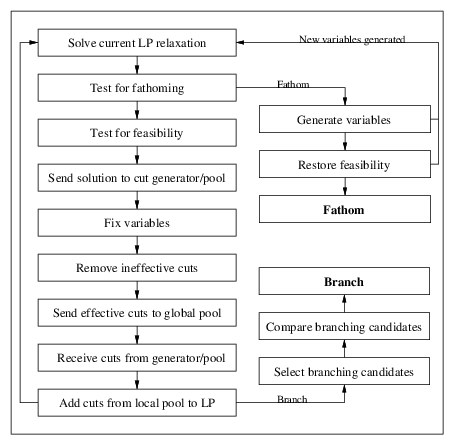
\includegraphics[width=4.8in]{lploop}
\caption{Overview of the node processing loop}
\label{LP-loop}
\end{figure}

\subsubsection{The LP Engine}

SYMPHONY requires the use of a third-party callable library (referred
to as the {\em LP engine} or {\em LP library}) to solve the LP
relaxations once they are formulated. As with the user functions,
SYMPHONY communicates with the LP engine through an API that converts
SYMPHONY's internal data structures into those of the LP engine.
Currently, the framework will only work with advanced, simplex-based
LP engines, such as CPLEX \cite{cplex}, since the LP engine must be
able to accept an advanced basis, and provide a variety of data to the
framework during the solution process. The internal data structures
used for maintaining the LP relaxations are similar to those of CPLEX
and matrices are stored in the standard column-ordered format.

\subsubsection{Managing the LP Relaxation}
\label{lp-relaxation}

The majority of the computational effort of BCP is spent
solving LPs and hence a major emphasis in the development was to make
this process as efficient as possible. Besides using a good LP engine,
the primary way in which this is done is by controlling the size of
each relaxation, both in terms of number of active variables and
number of active constraints. 

The number of constraints is controlled through use of a local
pool and through purging of ineffective constraints. When a cut is
generated by the cut generator, it is first sent to the local cut
pool. In each iteration, up to a specified number of the strongest
cuts (measured by degree of violation) from the local pool are added
to the problem. Cuts that are not strong enough to be added to the
relaxation are eventually purged from the list. In addition, cuts are
purged from the LP itself when they have been deemed ineffective for
more than a specified number of iterations, where ineffective is
defined as either (1) the corresponding slack variable is positive,
(2) the corresponding slack variable is basic, or (3) the dual value
corresponding to the row is zero (or very small). Cuts that have
remained effective in the LP for a specified number of iterations are
sent to the global pool where they can be used in later search nodes.
Cuts that have been purged from the LP can be made active again if
they later become violated.

The number of variables (columns) in the relaxation is controlled
through {\em reduced cost fixing} and {\em dynamic column generation}.
Periodically, each active variable is {\em priced} to see if it can be
fixed by reduced cost. That is, the LP reduced cost is examined in an
effort  to determine whether fixing that variable at
one of its bounds would remove improving solutions; if not, the
variable is fixed and removed from consideration. If the matrix is
{\em full} at the time of the fixing, meaning that all unfixed
variables are active, then the fixing is permanent for that subtree.
Otherwise, it is temporary and only remains in force until the next
time that columns are dynamically generated.

Because SYMPHONY was originally designed for combinatorial problems
with relatively small numbers of variables, techniques for performing
dynamic column generation are somewhat unrefined. Currently, variables
are priced out sequentially by index, which can be costly. To improve
the process of pricing variables, we plan to increase the symmetry
between our methods for handling variables and those for handling
cuts. This includes (1) allowing user-defined, abstract
representations for variables, (2) allowing the use of ``variable
generators'' analogous to cut generators, (3) implementing both global
and local pools for variables, (4) implementing heuristics that help
determine the order in which the indexed variables should be priced,
and (5) allowing for methods of simultaneously pricing out large
groups of variables. Much of this is already implemented in COIN/BCP.

Because pricing is computationally burdensome, it currently takes
place only either (1) before branching (optional), or (2) when a node
is about to be pruned (depending on the phase---see the description of
the two-phase algorithm in Sect. \ref{two-phase}). To use dynamic
column generation, the user must supply a subroutine which generates
the column corresponding to a particular user index, given the list of
active constraints in the current relaxation. When column generation
occurs, each column not currently active that has not been previously
fixed by reduced cost is either priced out immediately, or becomes
active in the current relaxation. Only a specified number of columns
may enter the problem at a time, so when that limit is reached, column
generation ceases. For further discussion of column generation, see
Sect. \ref{two-phase}, where the two-phase algorithm is described.

Since the matrix is stored in compressed form, considerable
computation may be needed to add and remove rows and columns. Hence,
rows and columns are only physically removed from the problem when
there are sufficiently many to make it ``worthwhile.'' Otherwise,
deleted rows and columns remain in the matrix but are simply ignored
by the computation. Note that because ineffective rows left in the
matrix increase the size of the basis unnecessarily, it is usually
advisable to adopt an aggressive strategy for row removal.

\subsubsection{Branching}
\label{branching}

Branching takes place whenever either (1) both cut generation and
column generation (if performed) have failed; (2) ``tailing off'' in
the objective function value has been detected; or (3) the
user chooses to force branching. Branching can take place on cuts or
variables and can be fully automated or fully controlled by the user,
as desired. Branching can result in as many children as the user
desires, though two is typical. Once it is decided that branching will
occur, the user must either select the list of candidates for {\em
strong branching} (see below for the procedure) or allow SYMPHONY to
do so automatically by using one of several built-in strategies, such
as branching on the variable whose value is farthest from being
integral. The number of candidates may depend on the level of the
current node in the tree---it is usually best to expend more effort on
branching near the top of the tree.

After the list of candidates is selected, each candidate is {\em
pre-solved}, by performing a specified number of iterations of the
dual simplex algorithm in each of the resulting subproblems. Based on
the objective function values obtained in each of the potential
children, the final branching object is selected, again either by the
user or by built-in rule. This procedure of using exploratory LP
information in this manner to select a branching candidate is commonly
referred to as {\em strong branching}. When the branching object has
been selected, the NP module sends a description of that object to the
tree manager, which then creates the children and adds them to the
list of candidate nodes. It is then up to the tree manager to specify
which node the now-idle NP module should process next. This issue is
further discussed below.

\subsection{The Tree Management Module}
\label{tree-management}

\subsubsection{Managing the Search Tree}

The tree manager's primary job is to control the execution of the
algorithm by deciding which candidate node should be chosen as the
next to be processed. This is done using either one of several
built-in rules or a user-defined rule. Usually, the goal of the search
strategy is to minimize overall running time, but it is sometimes
also important to find good feasible solutions early in the search
process. In general, there are two ways to decrease running
time---either by decreasing the size of the search tree or by
decreasing the time needed to process each search tree node.

To minimize the size of the search tree, the strategy is to select
consistently that candidate node with the smallest associated lower bound.
In theory, this strategy, sometimes called {\em best-first}, will lead
the smallest possible search tree. However, we need to consider the
time required to process each search tree node as well. This is affected
by both the quality of the current upper bound and by such factors as
communication overhead and node set-up costs. When considering these
additional factors, it is sometimes be more effective to deviate from the
best-first search order. We discuss the importance of such strategies
below.

\subsubsection{Search Chains and Diving}

One reason for not strictly enforcing the search order is because it
is somewhat expensive to construct a search node, send it to an NP
module, and set it up for processing. If, after branching, we choose
to continue processing one of the children of the current subproblem,
we avoid the set-up cost, as well as the cost of communicating the
node description of the retained child subproblem back to the tree
manager. This is called {\em diving} and the resulting chain of nodes
is called a {\em search chain}. There are a number of rules for
deciding when an NP module should be allowed to dive. One such rule is
to look at the number of variables in the current LP solution that
have fractional values. When this number is low, there may be a good
chance of finding a feasible integer solution quickly by diving. This
rule has the advantage of not requiring any global information. We
also dive if one of the children is ``close'' to being the best node,
where ``close'' is defined by a chosen parameter.

In addition to the time saved by avoiding reconstruction of the LP in
the child, diving has the advantage of often leading quickly to the
discovery of feasible solutions, as discussed above. Good upper bounds
not only allow earlier pruning of unpromising search chains, but also
should decrease the time needed to process each search tree node by
allowing variables to be fixed by reduced cost.

\subsubsection{The Two-Phase Algorithm}
\label{two-phase}

If no heuristic subroutine is available for generating feasible
solutions quickly, then a unique two-phase algorithm can also be
invoked. In the two-phase method, the algorithm is first run to
completion on a specified set of core variables. Any node that would
have been pruned in the first phase is instead sent to a pool of
candidates for the second phase. If the set of core variables is
small, but well-chosen, this first phase should be finished quickly
and should result in a near-optimal solution. In addition, the first
phase will produce a list of useful cuts. Using the upper bound and
the list of cuts from the first phase, the root node is {\em
repriced}---that is, it is reprocessed with the full set of variables
and cuts. The hope is that most or all of the variables not included
in the first phase will be priced out of the problem in the new root
node. Any variable thus priced out can be eliminated from the problem
globally. If we are successful at pricing out all of the inactive
variables, we have shown that the solution from the first phase was,
in fact, optimal. If not, we must go back and price out the (reduced)
set of extra variables in each leaf of the search tree produced during
the first phase. We then continue processing any node in which we fail
to price out all the variables.

In order to avoid pricing variables in every leaf of the tree, we can
{\em trim the tree} before the start of the second phase. Trimming the
tree consists of eliminating the children of any node for which
each child has lower bound above the current upper
bound. We then reprocess the parent node itself. This is typically
more efficient, since there is a high probability that, given the new
upper bound and cuts, we will be able to prune the parent node and
avoid the task of processing each child individually.

\subsection{The Cut Generation Module}

To implement the cut generator process, the user must provide a
function that accepts an LP solution and returns cuts violated by that
solution to the NP module. In parallel configurations, each cut is
returned immediately to the NP module, rather than being passed back
as a group once the function exits. This allows the LP to begin adding
cuts and solving the current relaxation before the cut generator is
finished if desired. Parameters controlling if and when the LP should
begin solving the relaxation before the cut generator is finished can
be set by the user.

SYMPHONY now generates generic cutting planes using the Cut Generator Library,
also available from 
\htmladdnormallink{COIN}{https://projects.coin-or.org/Cgl}
\begin{latexonly} 
COIN (\url{https://projects.coin-or.org/Cgl})
\end{latexonly}.
The CGL can be used to generate cuts in cases where problem-specific cutting
planes are not available or not implemented yet. 

\subsection{The Cut Management Module}

\subsubsection{Maintaining and Scanning the Pool}

The cut manager's primary job is to receive a solution from an
NP module and return cuts from the pool that are violated by it. The
cuts are stored along with two pieces of information---the level of
the tree on which the cut was generated, known simply as the {\em
level} of the cut, and the number of times it has been checked for
violation since the last time it was actually found to be violated,
known as the number of {\em touches}. The number of touches
can be used as a simplistic measure of its effectiveness. Since the pool
can get quite large, the user can choose to scan only cuts whose
number of touches is below a specified threshold and/or cuts that were
generated on a level at or above the current one in the tree. The idea
behind this second criterion is to try to avoid checking cuts that were
not generated ``nearby'' in the tree, as they are less likely to be
effective. Any cut generated at a level in the tree
below the level of the current node must have been generated in a
different part of the tree. Although this is admittedly a naive
method, it does seem to work reasonably well.

On the other hand, the user may define a specific measure of quality for
each cut to be used instead. For example, the degree of
violation is an obvious candidate. This measure of quality must be
computed by the user, since the cut pool module has no knowledge of
the cut data structures. The quality is recomputed every time
the user checks the cut for violation and a running average is used as
the global quality measure. The cuts in the pool are periodically
sorted by this measure and only the highest quality cuts
are checked each time. All duplicate cuts, as well as all cuts whose
number of touches exceeds or whose quality falls below specified
thresholds, are periodically purged from the pool to keep it as small as
possible.

\subsubsection{Using Multiple Pools}
\label{multi-cut-pools}

For several reasons, it may be desirable to have multiple cut pools.
When there are multiple cut pools, each pool is initially assigned
to a particular node in the search tree. After being assigned to that
node, the pool services requests for cuts from that node and all
of its descendants until such time as one of its descendants gets
assigned to another cut pool. After that, it continues to
serve all the descendants of its assigned node that are not assigned
to other cut pools.

Initially, the first cut pool is assigned to the root node. All other cut
pools are unassigned. During execution, when a new node is sent to be
processed, the tree manager must determine which cut pool the node should be
serviced by. The default is to use the same cut pool as its parent. However,
if there is currently an idle cut pool process (either it has never been
assigned to any node or all the descendants of its assigned node have been
processed or reassigned), then that cut pool is assigned to this new node. All
the cuts currently in the cut pool of its parent node are copied to the new
pool to initialize it, after which the two pools operate independently on
their respective subtrees. When generating cuts, the NP module sends the new
cuts to the cut pool assigned to service the node during whose processing the
cuts were generated.

The primary motivation behind the idea of multiple cut pools is
two-fold. First, we want simply to limit the size of each pool as
much as possible. By limiting the number of nodes that a cut pool has
to service, the number of cuts in the pool will be similarly limited.
This not only allows cut storage to spread over multiple processors,
and hence increases the available memory, but at the same time, the
efficiency with which the cut pool can be scanned for violated cuts is
also increased. A secondary reason for maintaining multiple cut pools is
that it allows us to limit the scanning of cuts to only those that
were generated in the same subtree as the current search node. As
described above, this helps focus the search and should increase the
efficiency and effectiveness of the search. This idea also
allows us to generate locally valid cuts, such as the classical
Gomory cuts (see \cite{nemwol88}).

\section{Parallelizing BCP}
\label{parallelizing}

Because of the clear partitioning of work that occurs when the
branching operation generates new subproblems, branch and bound
algorithms lend themselves well to parallelization. As a result, there
is already a significant body of research on performing branch and
bound in parallel environments. We again point the reader to the
survey of parallel branch and bound algorithms by Gendron and Crainic
\cite{gend:paral}, as well as other references such as
\cite{PICO,GraKum99,kuma:para4,kuma:para3}.

In parallel BCP, as in general branch and bound, there are two major
sources of parallelism. First, it is clear that any number of
subproblems on the current candidate list can be processed
simultaneously. Once a subproblem has been added to the list, it can
be properly processed before, during, or after the processing of any
other subproblem. This is not to say that processing a particular node
at a different point in the algorithm won't produce different
results---it most certainly will---but the algorithm will terminate
correctly in any case. The second major source of parallelism is to
parallelize the processing of individual subproblems. By allowing
separation to be performed in parallel with the solution of the linear
programs, we can theoretically process a node in little more than the
amount of time it takes to solve the sequence of LP relaxations. Both
of these sources of parallelism can be easily exploited using the
\BB\ framework.

The most straightforward parallel implementation, which is the one we
currently employ, is a master-slave model, in which there is a central
manager responsible for partitioning the work and parceling it out to
the various slave processes that perform the actual computation. The
reason we chose this approach is because it allows memory-efficient
data structures for sequential computation and yet is conceptually
easy to parallelize. Unfortunately, this approach does have limited
scalability. For further discussions on the scalability of BCP algorithms and
approaches to improving it, see \cite{symphony1} and \cite{ALPS2}.

%\subsection{Details of the Parallel Implementation}

\subsection{Parallel Configurations}

SYMPHONY supports numerous configurations, ranging from completely
sequential to fully parallel, allowing efficient execution in many
different computational settings. As described in the previous
section, there are five modules in the standard distributed
configuration. Various subsets of these modules can be
combined to form separate executables capable of communicating
with each other across a network. When two or more modules are combined,
they simply communicate through shared-memory instead of through
message-passing. However, they are also forced to run in sequential
fashion in this case, unless the user chooses to enable threading
using an OpenMP compliant compiler (see next section). 

As an example, the default distributed configuration includes a
separate executable for each module type, allowing full parallelism.
However, if cut generation is fast and not memory-intensive,
it may not be worthwhile to have the NP module and its associated cut
generator work independently, as this increases communication
overhead without much potential benefit. In this case, the cut
generator functions can be called directly from the NP module,
creating a single, more efficient executable.

\subsection{Inter-process Communication}

SYMPHONY can utilize any third-party communication protocol supporting basic
message-passing functions. All communication subroutines interface with
SYMPHONY through a separate communications API. Currently, PVM \cite{PVMbook}
is the only message-passing protocol supported, but interfacing with another
protocol is a straightforward exercise.

Additionally, it is possible to configure the code to run in parallel using
threading to process multiple search tree nodes simultaneously. Currently,
this is implemented using OpenMP compiler directives to specify the parallel
regions of the code and perform memory locking functions. Compiling the code
with an OpenMP compliant compiler will result in a shared-memory parallel
executable. For a list of OpenMP compliant compilers and other resources,
visit \code{\url{http://www.openmp.org}}.

\subsection{Fault Tolerance}
\label{fault-tolerance} 

Fault tolerance is an important consideration for solving large problems on
computing networks whose nodes may fail unpredictably. The tree manager tracks
the status of all processes and can restart them as necessary. Since the state
of the entire tree is known at all times, the most that will be lost if an NP
module or cut generator is killed is the work that had been completed on that
particular search node. To protect against the tree manager itself or a cut
pool being killed, full logging capabilities have been implemented. If
desired, the tree manager can write out the entire state of the tree to disk
periodically, allowing a warm restart if a fault occurs. Similarly, the cut
pool process can be warm-started from a log file. This not only allows for
fault tolerance but also for full reconfiguration in the middle of solving a
long-running problem. Such reconfiguration could consist of anything from
adding more processors to moving the entire solution process to another
network.

